\section{Final Concept}

The final basic geometry of our final concept is shown in figure \ref{fig:final_concept}. It is important to note that the render does not include all components such as the propellant feed system and propellant diffuser, and that the design may very well change as we move through the design process. However, it does the job of conveying some of the design goals and choices that have been made. The final concept will consist of the following features:

\begin{enumerate}
    \item Magnetic Field System - will consist of a ferromagnetic core with permanent magnets to create the required magnetic field topology. This will reduce power consumption and
    avionics system complexity
    \item Cathode - will be centrally mounted on the thruster axis allowing for a more compact design
    \item Ring anode - simple and well understood design
    \item Propellant feed system - will consist of a pressure vessel, custom propellant diffuser, and supporting hardware. May become to primary conductor to the anode.
\end{enumerate}

\begin{figure}[H]
    \centering
    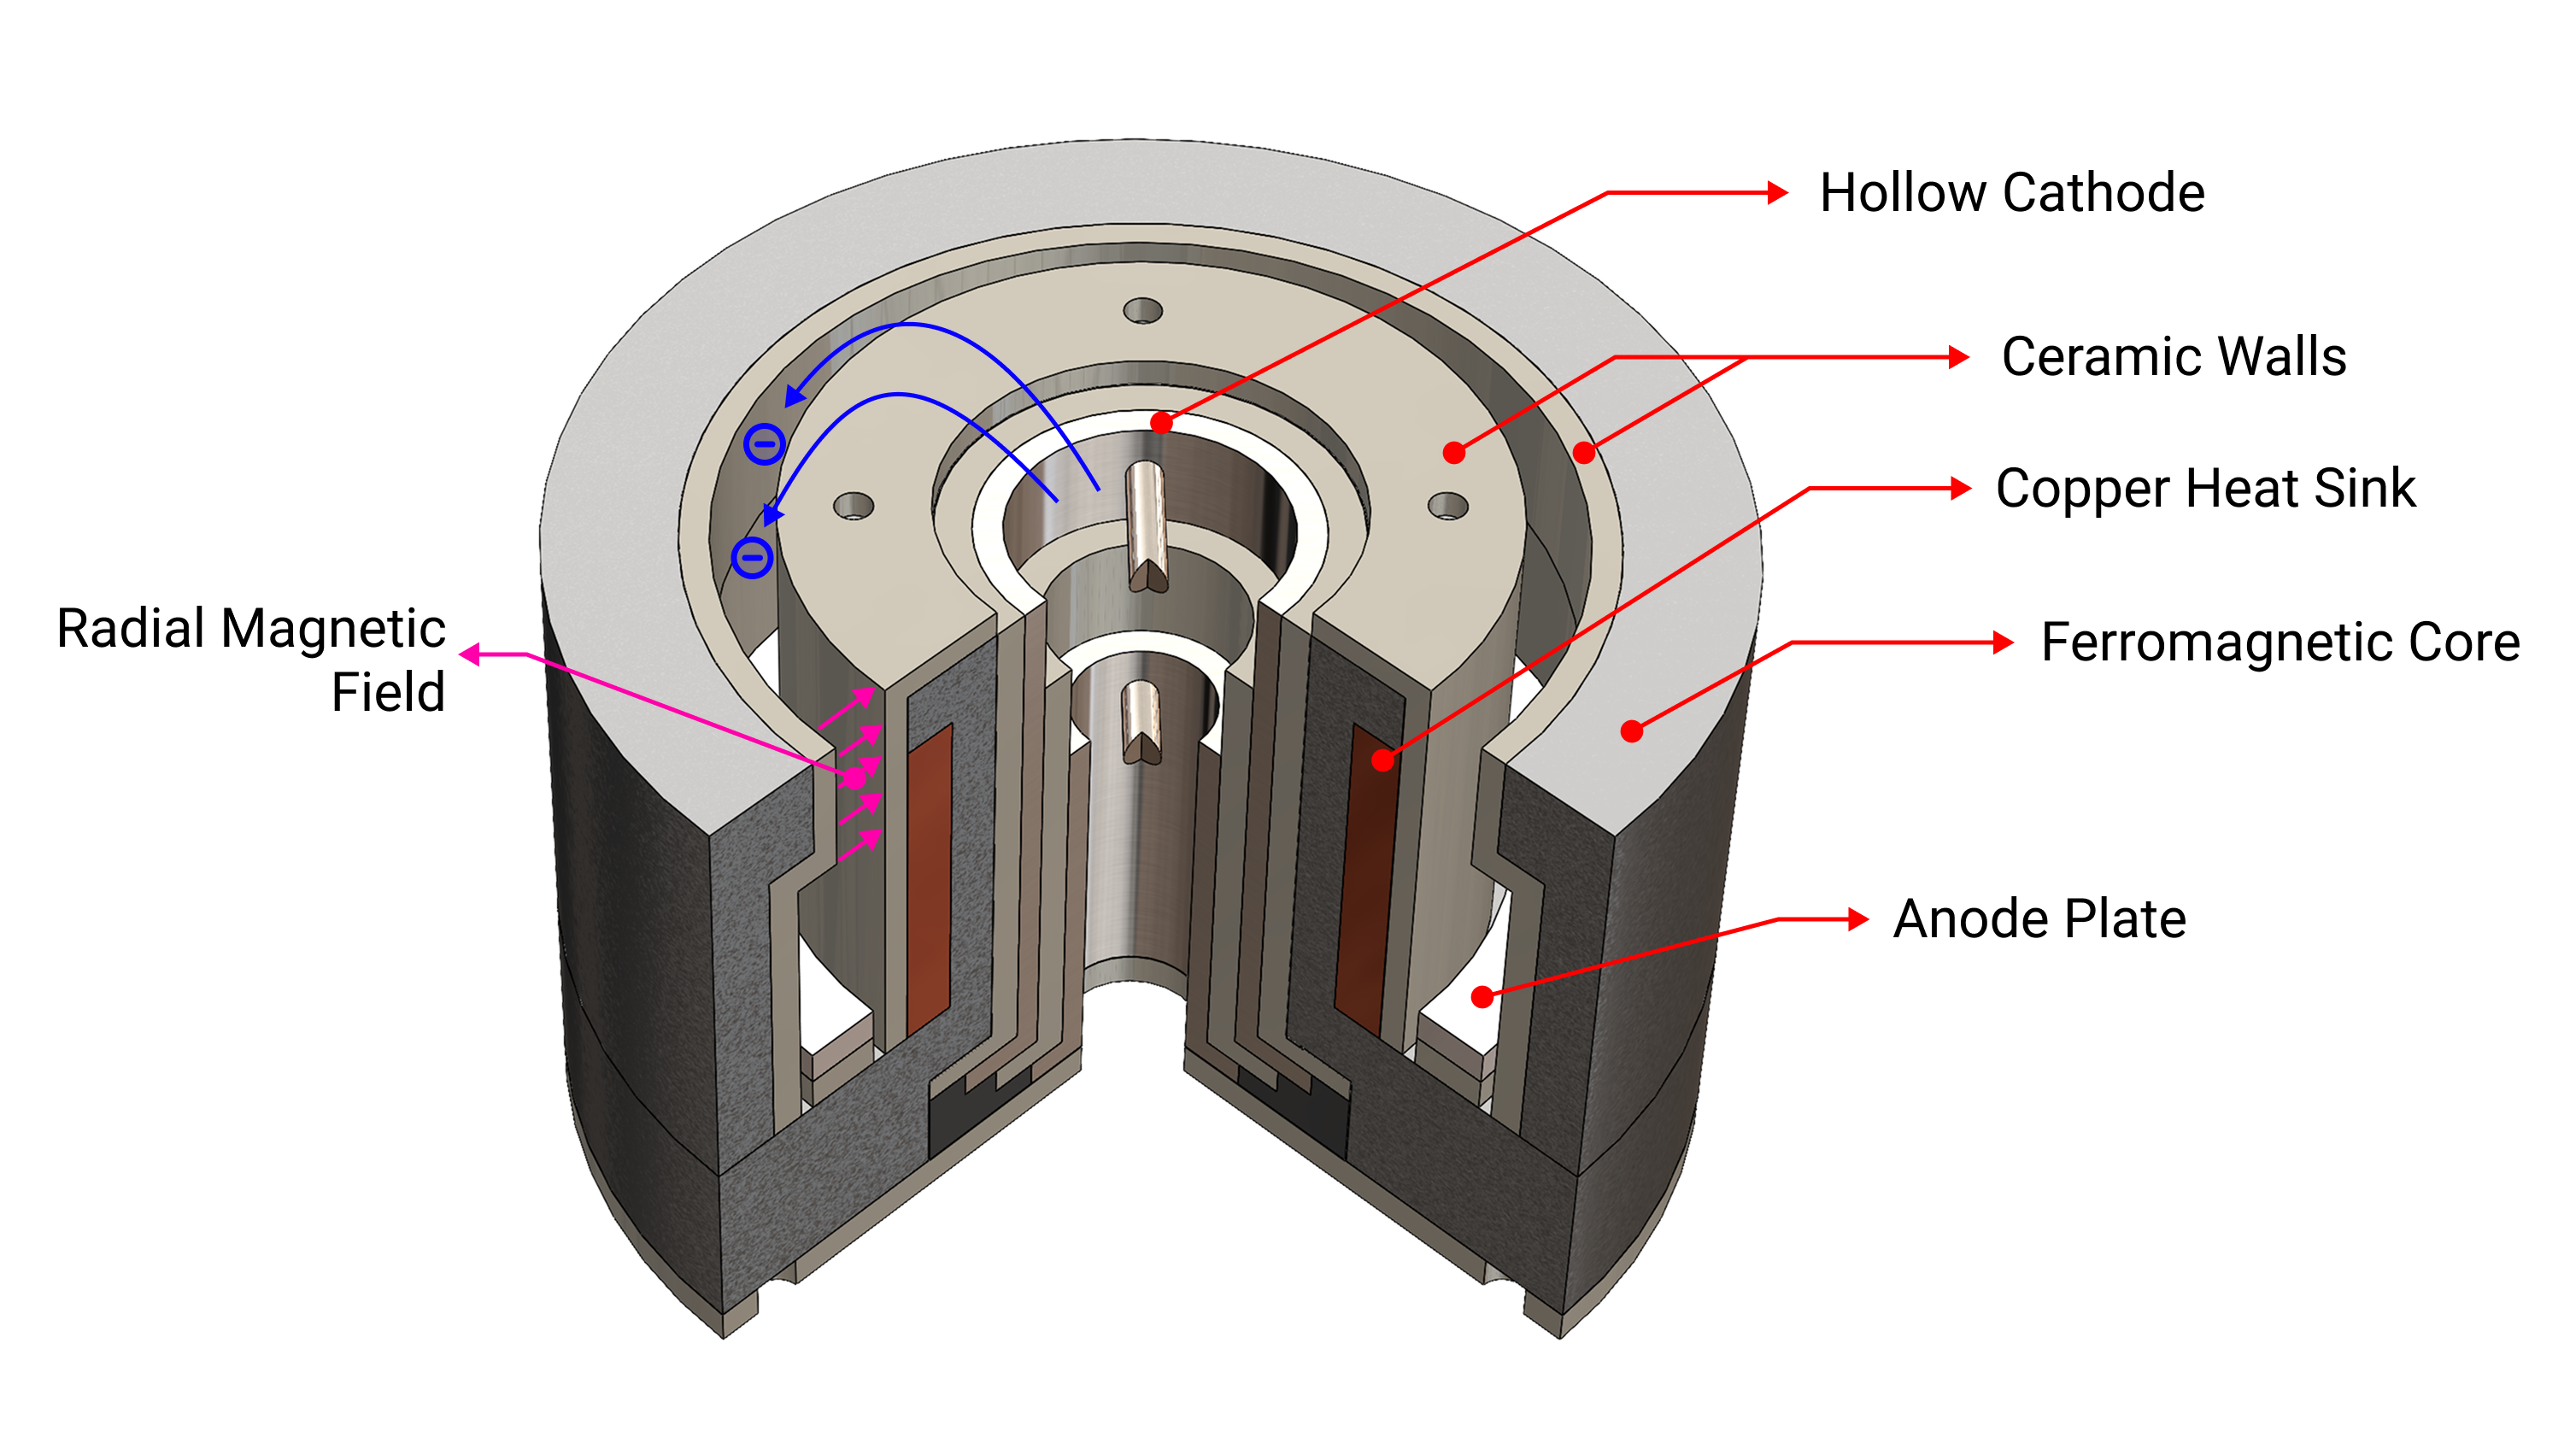
\includegraphics[width=1.0\textwidth]{images/Concepts/final concept.png}
    \captionsetup{justification=centering}
    \caption{Final Concept Diagram}
    \label{fig:final_concept}
\end{figure}